\documentclass[11pt,a4paper]{article}

\usepackage[margin=20mm,top=22mm,bottom=23mm]{geometry}
\usepackage{fontspec}
\usepackage{microtype}
\usepackage{graphicx}
\usepackage{booktabs}
\usepackage{tabularx}
\usepackage{longtable}
\usepackage{array}
\usepackage{enumitem}
\usepackage[table]{xcolor}
\usepackage{tikz}
\usetikzlibrary{positioning}
\usepackage[most]{tcolorbox}
\usepackage{fancyhdr}
\usepackage{titlesec}
\usepackage{hyperref}
\usepackage{xurl}
\usepackage{lastpage}
\usepackage{ragged2e}
\usepackage{setspace}
\usepackage{needspace}
\usepackage{etoolbox}
\usepackage{tocloft}

\setmainfont{Baskerville}
\setsansfont{Avenir Next}
\setmonofont{Menlo}

\definecolor{NordNavy}{HTML}{0B1B3F}
\definecolor{NordBlue}{HTML}{1A3DBC}
\definecolor{NordGold}{HTML}{C8A96A}
\definecolor{NordPaper}{HTML}{F5F1E8}
\definecolor{NordPaperTwo}{HTML}{ECE6DA}
\definecolor{NordInk}{HTML}{172033}
\definecolor{NordMuted}{HTML}{626A78}
\definecolor{NordGreen}{HTML}{2E7D61}
\definecolor{NordRed}{HTML}{A64646}
\definecolor{NordAmber}{HTML}{A56A20}

\hypersetup{
  colorlinks=true,
  linkcolor=NordBlue,
  urlcolor=NordBlue,
  citecolor=NordBlue,
  pdftitle={Kostenanalyse und Preisstrategie für den Betrieb von svnord.de},
  pdfauthor={Alperen Adatepe},
  pdfsubject={Vertrauliche Kalkulation, Stand 22. August 2026}
}
\urlstyle{same}

\setlength{\parindent}{0pt}
\setlength{\parskip}{5.5pt}
\setlength{\emergencystretch}{2em}
\renewcommand{\arraystretch}{1.32}
\setlist[itemize]{leftmargin=5mm,itemsep=2pt,topsep=3pt}
\setlist[enumerate]{leftmargin=6mm,itemsep=2pt,topsep=3pt}
\widowpenalty=10000
\clubpenalty=10000
\displaywidowpenalty=10000
\raggedbottom
\setcounter{tocdepth}{1}
\setcounter{secnumdepth}{2}

\renewcommand{\contentsname}{Berichtsstruktur}
\renewcommand{\cfttoctitlefont}{\sffamily\large\bfseries\color{NordNavy}}
\renewcommand{\cftsecfont}{\sffamily\small\color{NordInk}}
\renewcommand{\cftsecpagefont}{\sffamily\small\bfseries\color{NordBlue}}
\setlength{\cftbeforesecskip}{2.2pt}
\setlength{\cftsecindent}{0pt}
\setlength{\cftsecnumwidth}{8mm}

\titleformat{\section}
  {\sffamily\Large\bfseries\color{NordNavy}}
  {\colorbox{NordGold}{\makebox[8mm][c]{\color{NordNavy}\thesection}}}{0.7em}{}
\titleformat{\subsection}
  {\sffamily\large\bfseries\color{NordBlue}}
  {\thesubsection}{0.6em}{}
\titlespacing*{\section}{0pt}{15pt}{7pt}
\titlespacing*{\subsection}{0pt}{11pt}{4pt}
\pretocmd{\section}{\Needspace{8\baselineskip}}{}{}
\pretocmd{\subsection}{\Needspace{5\baselineskip}}{}{}

\pagestyle{fancy}
\fancyhf{}
\fancyhead[L]{\sffamily\footnotesize\color{NordMuted}SV Nord München-Lerchenau e.V.}
\fancyhead[R]{\sffamily\footnotesize\color{NordMuted}Vertrauliche Kostenanalyse}
\fancyfoot[L]{\sffamily\footnotesize\color{NordMuted}Stand 22.08.2026}
\fancyfoot[R]{\sffamily\footnotesize\color{NordMuted}Seite \thepage\ von \pageref{LastPage}}
\renewcommand{\headrulewidth}{0.25pt}
\renewcommand{\footrulewidth}{0pt}

\newcolumntype{Y}{>{\RaggedRight\arraybackslash}X}
\newcolumntype{L}[1]{>{\RaggedRight\arraybackslash}p{#1}}
\newcolumntype{R}[1]{>{\RaggedLeft\arraybackslash}p{#1}}

\newtcolorbox{summarybox}[1][]{
  enhanced,
  colback=NordPaper,
  colframe=NordGold,
  boxrule=0.7pt,
  arc=2mm,
  left=5mm,right=5mm,top=4mm,bottom=4mm,
  #1
}

\newtcolorbox{riskbox}[1][]{
  enhanced,
  colback=NordRed!5,
  colframe=NordRed!70,
  boxrule=0.6pt,
  arc=1.5mm,
  left=4mm,right=4mm,top=3mm,bottom=3mm,
  #1
}

\newtcolorbox{decisionbox}[1][]{
  enhanced,
  colback=NordBlue!5,
  colframe=NordBlue!70,
  boxrule=0.7pt,
  arc=2mm,
  left=5mm,right=5mm,top=4mm,bottom=4mm,
  #1
}

\newtcolorbox{metricbox}[1][]{
  enhanced,
  colback=white,
  colframe=NordPaperTwo,
  boxrule=0.5pt,
  arc=2mm,
  left=3.5mm,right=3.5mm,top=3mm,bottom=3mm,
  height=28mm,
  #1
}

\newcommand{\statusok}{\textcolor{NordGreen}{\sffamily\bfseries bestätigt}}
\newcommand{\statusassumed}{\textcolor{NordAmber}{\sffamily\bfseries Annahme}}
\newcommand{\statusrisk}{\textcolor{NordRed}{\sffamily\bfseries Risiko}}
\newcommand{\eur}[1]{#1\,€}
\newcommand{\usd}[1]{#1\,US\$}

\begin{document}
\hypersetup{pageanchor=false}

\begin{titlepage}
  \pagecolor{NordNavy}
  \color{white}
  \begin{tikzpicture}[remember picture,overlay]
    \fill[NordGold] (current page.north west) rectangle ([xshift=8mm]current page.south west);
    \fill[NordBlue] ([xshift=8mm]current page.north west) rectangle ([xshift=11mm]current page.south west);
    \draw[NordGold!35,line width=0.4pt]
      ([xshift=24mm,yshift=-26mm]current page.north west)
      -- ([xshift=-20mm,yshift=-26mm]current page.north east);
  \end{tikzpicture}

  \vspace*{8mm}
  \begin{minipage}[t]{0.68\textwidth}
    {\sffamily\footnotesize\bfseries\color{NordGold}\MakeUppercase{Betrieb, Infrastruktur und Preisstrategie}}\\[10mm]
    {\sffamily\fontsize{29}{33}\selectfont\bfseries
      Kostenanalyse\\[2mm]
      \color{NordGold}SV Nord Website}
  \end{minipage}
  \hfill
  \begin{minipage}[t]{0.21\textwidth}
    \raggedleft
    
\includegraphics[width=27mm]{public/svnord-logo.png}
  \end{minipage}

  \vfill

  \begin{minipage}{0.86\textwidth}
    {\sffamily\Large\bfseries Laufende Kosten, Wachstumsszenarien und monatliches Preismodell}\\[4mm]
    {\large Ausführliche interne Entscheidungsgrundlage für den Betrieb von \texttt{www.svnord.de}}
  \end{minipage}

  \vfill

  
\begin{tikzpicture}
    \node[fill=NordGold,text=NordNavy,rounded corners=2pt,inner xsep=10pt,inner ysep=6pt,
      font=\sffamily\bfseries] {EMPFEHLUNG: \eur{49,00} NETTO PRO MONAT};
  \end{tikzpicture}

  \vspace{13mm}
  {\sffamily\small
    \begin{tabular}{@{}ll@{}}
      Auftraggeber & Alperen Adatepe \\
      Projekt & \texttt{nord-lerchenau} \\
      Stand & 22. August 2026 \\
      Klassifizierung & Vertraulich, nur zur internen Kalkulation \\
    \end{tabular}
  }
  \vspace*{5mm}
\end{titlepage}

\hypersetup{pageanchor=true}
\nopagecolor
\color{NordInk}

{\sffamily\footnotesize\bfseries\color{NordBlue}\MakeUppercase{Management Summary}}\\[2mm]
{\sffamily\LARGE\bfseries\color{NordNavy}Entscheidung in 60 Sekunden}

\vspace{3mm}
\noindent
\begin{minipage}[t]{0.315\textwidth}
  \begin{metricbox}
    {\sffamily\scriptsize\bfseries\color{NordMuted}\MakeUppercase{Kundenpreis}}\\[1.5mm]
    {\sffamily\fontsize{23}{25}\selectfont\bfseries\color{NordNavy}\eur{49}}\\[-0.5mm]
    {\sffamily\scriptsize\color{NordMuted}netto pro Monat}
  \end{metricbox}
\end{minipage}\hfill
\begin{minipage}[t]{0.315\textwidth}
  \begin{metricbox}
    {\sffamily\scriptsize\bfseries\color{NordMuted}\MakeUppercase{Kostenbudget}}\\[1.5mm]
    {\sffamily\fontsize{23}{25}\selectfont\bfseries\color{NordBlue}\eur{18}}\\[-0.5mm]
    {\sffamily\scriptsize\color{NordMuted}externer Mittelabfluss}
  \end{metricbox}
\end{minipage}\hfill
\begin{minipage}[t]{0.315\textwidth}
  \begin{metricbox}
    {\sffamily\scriptsize\bfseries\color{NordMuted}\MakeUppercase{Interner Anteil}}\\[1.5mm]
    {\sffamily\fontsize{23}{25}\selectfont\bfseries\color{NordGreen}\eur{27}}\\[-0.5mm]
    {\sffamily\scriptsize\color{NordMuted}vor Steuern und Zeit}
  \end{metricbox}
\end{minipage}

\begin{summarybox}
  Die Website arbeitet heute mit sehr kleinen Datenmengen und überwiegend kostenlosen Tarifen. Für einen bezahlten Kundenbetrieb ist der Vercel-Hobby-Tarif jedoch keine belastbare Grundlage, weil Vercel ihn für persönliche und nicht kommerzielle Nutzung vorsieht.

  Die wirtschaftlich saubere Basis ist deshalb \textbf{Vercel Pro zu \usd{20} monatlich}. Beim ECB-Referenzkurs vom 21.08.2026 entspricht das rund \eur{17,10}. Zusammen mit normaler OpenAI-Nutzung wird ein externes Budget von \eur{18} angesetzt. Eine Reserve von \eur{4} fängt kleine Verbrauchs- und Währungsschwankungen auf.

  Der empfohlene Preis von \textbf{\eur{49 netto pro Monat}} ist damit niedrig genug für den Verein und robust genug für einen professionellen Betrieb. Bei 19 Prozent Umsatzsteuer läge der Zahlbetrag bei \eur{58,31}. Der verbleibende Anteil ist ein Deckungsbeitrag vor Steuern und vor Bewertung der eigenen Arbeitszeit.
\end{summarybox}

\vspace{-2mm}
\tableofcontents
\newpage

\section{Auftrag, Umfang und Methode}

Ziel ist eine belastbare Antwort auf vier Fragen:

\begin{enumerate}
  \item Welche technischen Dienste erzeugen heute oder später laufende Kosten?
  \item Wie hoch sind diese Kosten bei normaler Nutzung und bei Wachstum?
  \item Welcher Monatspreis deckt Anbieterrechnungen, Schwankungen und einen sinnvollen persönlichen Anteil?
  \item Wie wird dieser Preis dem Kunden erklärt, ohne die interne Marge offenzulegen?
\end{enumerate}

Die Analyse basiert auf drei Evidenzarten:

\begin{itemize}
  \item \textbf{Repository-Evidenz:} Produktionspfade, Umgebungsvariablen, API-Routen, Cache-Strategien und Abhängigkeiten im aktuellen Worktree.
  \item \textbf{Produktivmessungen:} Vercel-Projekt und Tarif, Blob-Bestand sowie aggregierte Größe der Neon-Datenbank. Es wurden keine personenbezogenen Inhalte gelesen.
  \item \textbf{Aktuelle Primärquellen:} offizielle Preis- und Produktseiten der Anbieter, abgerufen am 22.08.2026.
\end{itemize}

Nicht Bestandteil der Monatsrechnung sind neue Funktionen, redaktionelle Arbeiten, größere Fehlerbehebungen, Rechts- oder Steuerberatung sowie Kosten für Domains und bestehende Mailpostfächer des Vereins. Diese Punkte werden getrennt behandelt.

\section{Ist-Architektur und Kostenpfade}

\subsection{Technische Lieferkette}

\begin{center}
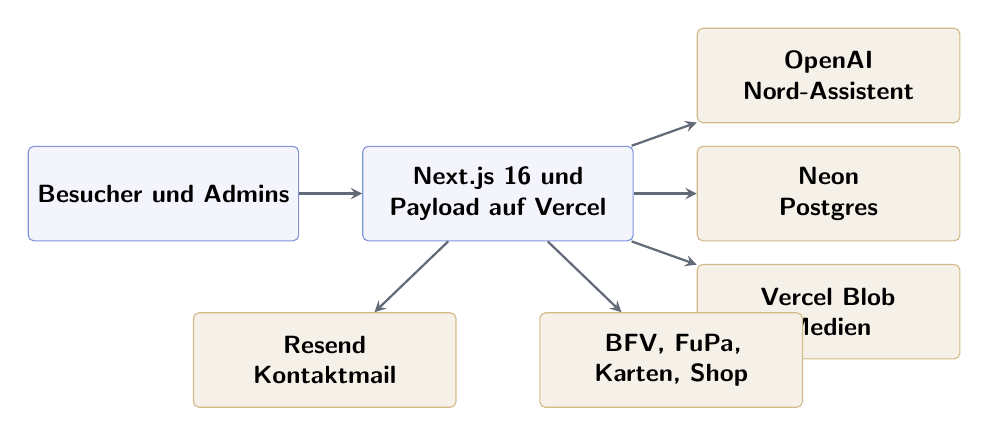
\begin{tikzpicture}[
  node distance=9mm and 8mm,
  box/.style={rounded corners=2pt,draw=NordBlue!55,fill=NordBlue!5,
    minimum height=12mm,text width=32mm,align=center,font=\sffamily\small\bfseries},
  ext/.style={rounded corners=2pt,draw=NordGold!80,fill=NordPaper,
    minimum height=12mm,text width=31mm,align=center,font=\sffamily\small\bfseries},
  arr/.style={-stealth,thick,draw=NordMuted}
]
  \node[box] (visitor) {Besucher und Admins};
  \node[box,right=of visitor] (vercel) {Next.js 16 und Payload auf Vercel};
  \node[ext,right=of vercel,yshift=15mm] (openai) {OpenAI\\Nord-Assistent};
  \node[ext,right=of vercel,yshift=0mm] (neon) {Neon\\Postgres};
  \node[ext,right=of vercel,yshift=-15mm] (blob) {Vercel Blob\\Medien};
  \node[ext,below=of vercel,xshift=-22mm] (resend) {Resend\\Kontaktmail};
  \node[ext,below=of vercel,xshift=22mm] (freeapis) {BFV, FuPa, Karten, Shop};
  \draw[arr] (visitor) -- (vercel);
  \draw[arr] (vercel) -- (openai);
  \draw[arr] (vercel) -- (neon);
  \draw[arr] (vercel) -- (blob);
  \draw[arr] (vercel) -- (resend);
  \draw[arr] (vercel) -- (freeapis);
\end{tikzpicture}
\end{center}

Die gesamte Anwendung ist eine gemeinsame Next.js-Anwendung. Payload CMS läuft nicht als separater SaaS-Dienst, sondern innerhalb desselben Deployments. Daraus entstehen keine Payload-Lizenzkosten, jedoch Serverless-Rechenzeit, Datenbankzugriffe und permanenter Medienspeicher.

\Needspace{18\baselineskip}
\subsection{Bestätigter Produktivbestand}

\begin{tabularx}{\textwidth}{L{35mm}Y L{32mm}}
  \toprule
  \rowcolor{NordNavy}
  \color{white}\sffamily\bfseries Messpunkt &
  \color{white}\sffamily\bfseries Ergebnis &
  \color{white}\sffamily\bfseries Evidenz \\
  Vercel-Projekt & \texttt{nord-lerchenau}, produktiv, Fluid Compute, Funktionen in \texttt{iad1} & \statusok \\
  Vercel-Tarif & Hobby, aktive Abrechnung zu \eur{0} & \statusok \\
  Blob-Speicher & 486 Objekte, 28.408.192 Byte, rund 28,4 MB & \statusok \\
  Neon Postgres & 12 MB Datenbankgröße, 47 Tabellen, rund 3,8 MB Relationsdaten & \statusok \\
  OpenAI-Modell & Standardwert \texttt{gpt-4o-mini} & \statusok \\
  OpenAI-Limits im Code & höchstens 20 Nachrichten, 4.000 Zeichen je Nachricht, 600 Ausgabetoken & \statusok \\
  Neon-Tarif & Free laut Projektdokumentation, keine aktuelle Kontorechnung eingesehen & \statusassumed \\
  Resend-Tarif & Free als Kalkulationsannahme, keine aktuelle Kontorechnung eingesehen & \statusassumed \\
  \bottomrule
\end{tabularx}

\begin{riskbox}
  \textbf{Wichtige Kontenlage.} Laut aktuellem Übergabestatus liegen Server, Datenbank, Bildspeicher, Mailversand und Assistent auf Entwicklerkonten. Domain und Postfach liegen beim Verein. Diese Konstellation ist günstig und schnell, erhöht aber das Ausfall- und Übergaberisiko. Die Monatsvereinbarung sollte Kontenverantwortung, Zahlungsweg, Zugriff und Kündigungsübergabe ausdrücklich regeln.
\end{riskbox}

\section{Einzelanalyse aller laufenden Komponenten}

\subsection{Vercel: Hosting, Deployment und Serverless-Funktionen}

\textbf{Heutiger Zustand:} Hobby zu \eur{0}. Der Tarif enthält unter anderem bis zu eine Million Function Invocations, vier CPU-Stunden, 360 GB-Stunden provisionierten Speicher und 100 GB Fast Data Transfer. Bei Überschreitung kann die Hobby-Anwendung pausiert werden.

\textbf{Vertragliches Problem:} Vercel beschreibt Hobby als Tarif für persönliche, nicht kommerzielle Nutzung. Sobald die Anwendung als bezahlter Kundenbetrieb geführt wird, ist Hobby keine belastbare Kalkulationsgrundlage. Ob die Vereinswebsite selbst gemeinnützig ist, löst die Frage nach dem professionell erbrachten und abgerechneten Betrieb nicht eindeutig.

\textbf{Empfehlung:} Vercel Pro zu \usd{20} pro Monat. Darin sind ein Deploying Seat und \usd{20} monatliches Nutzungsguthaben enthalten. Fast Data Transfer bis 1 TB und zehn Millionen Edge Requests sind vor einer zusätzlichen Belastung enthalten. Für dieses Projekt ist deshalb im normalen Betrieb nur die feste Plattformgebühr zu erwarten.

\textbf{Budgetwert:} \eur{17,10} zum ECB-Kurs, in der internen Monatsplanung auf \eur{17,50} gerundet.

\subsection{Vercel Blob: Bilder und CMS-Uploads}

Der Blob-Store ist produktiv erforderlich, weil der Verein Bilder im Payload-Admin hochladen und ersetzen kann. Der reale Bestand von 28,4 MB ist sehr klein. Selbst bei einer Verzehnfachung auf rund 284 MB bleibt der Speicherverbrauch niedrig.

Vercel nennt für Blob regional ungefähr \usd{0,023} bis \usd{0,041} pro GB und Monat, \usd{0,05} bis \usd{0,117} pro GB Blob-Datentransfer sowie separate Sätze für Operationen. Diese Nutzung fällt auf Pro zuerst in das monatliche Nutzungsguthaben. Beim aktuellen Bestand ist der reine Speicherwert deutlich kleiner als ein Cent pro Monat. Relevanter wäre ein plötzlich stark ansteigender Bildtransfer.

\textbf{Budgetwert im Normalszenario:} innerhalb des Vercel-Pro-Guthabens, kein zusätzlicher Mittelabfluss.

\subsection{Neon Postgres: CMS, Kontaktanfragen und Inhalte}

Die Datenbank ist die zentrale Quelle für Teams, Beiträge, Sponsoren, Medienmetadaten, Kontaktanfragen und globale Seiteneinstellungen. Die gemessenen 12 MB nutzen nur rund 2,4 Prozent des Free-Speicherlimits von 0,5 GB.

Der aktuelle Neon-Free-Tarif nennt 100 CU-Stunden und 0,5 GB Speicher pro Projekt, maximal 2 CU und ein Wiederherstellungsfenster von sechs Stunden. Compute skaliert nach Inaktivität auf null. Das passt technisch sehr gut zur ungleichmäßigen Last einer Vereinswebsite.

\textbf{Kosten heute:} voraussichtlich \eur{0}. Die genaue CU-Nutzung konnte ohne neue Neon-Kontoanmeldung nicht verifiziert werden.

\textbf{Wachstumsoption:} Neon Launch ist verbrauchsabhängig. Offiziell werden \usd{0,106} pro CU-Stunde und \usd{0,35} pro GB und Monat genannt. Neon zeigt für eine intermittierende Last mit 140 CU-Stunden und 1 GB einen typischen Betrag von rund \usd{15} monatlich. Für diese Anwendung wäre der reale Betrag wegen der kleinen Datenbank vermutlich niedriger, sofern der Compute weiterhin regelmäßig auf null skaliert.

\begin{riskbox}
  \textbf{Sicherungsrisiko.} Sechs Stunden Time Travel sind kein unabhängiges Langzeitbackup. Aktuell ist keine eigene, geprüfte Datenbanksicherung dokumentiert. Ein monatlicher Preis darf erst dann mit „Backup inklusive“ beworben werden, wenn ein automatischer Dump, verschlüsselte Ablage und ein Wiederherstellungstest tatsächlich eingerichtet sind.
\end{riskbox}

\subsection{Resend: Kontaktformular und Zustellung}

Das Kontaktformular speichert Anfragen in Payload und versendet zusätzlich eine E-Mail über Resend. Der Free-Tarif enthält 3.000 transaktionale E-Mails im Monat und höchstens 100 pro Tag. Für den normalen Vereinsbetrieb ist das großzügig.

\textbf{Kosten heute:} voraussichtlich \eur{0}. Das aktuelle Projekt verwendet interimistisch ein Entwicklerkonto und eine Entwicklerdomain als Absender. Ein vereinseigenes Resend-Konto und die Verifizierung von \texttt{svnord.de} sind noch eine organisatorische Aufgabe.

\textbf{Upgrade-Schwelle:} Resend Pro kostet \usd{20} monatlich für 50.000 E-Mails. Dieser Schritt wäre erst bei erheblich größerem Versand oder zusätzlichen Anforderungen sinnvoll.

\subsection{OpenAI: Nord-Assistent}

Der öffentliche Endpunkt \texttt{/api/chat} verwendet standardmäßig \texttt{gpt-4o-mini}. Offiziell kostet das Modell \usd{0,15} je eine Million Eingabetoken und \usd{0,60} je eine Million Ausgabetoken.

Der Systemprompt umfasst im Repository 8.487 Byte. Für die Normalkalkulation werden 2.400 Eingabetoken und 160 Ausgabetoken je Antwort angesetzt. Daraus ergibt sich:

\begin{center}
  \fbox{\sffamily\bfseries
    Kosten je normale Antwort =
    $\frac{2.400 \times 0{,}15 + 160 \times 0{,}60}{1.000.000}$
    = \usd{0,000456}}
\end{center}

Beim ECB-Kurs entspricht das rund \eur{0,000390} pro normaler Antwort. Die KI selbst ist damit nicht der größte Kostenblock. Das eigentliche Risiko ist missbräuchlicher automatisierter Traffic.

\begin{tabularx}{\textwidth}{L{37mm}R{30mm}R{30mm}Y}
  \toprule
  \rowcolor{NordNavy}
  \color{white}\sffamily\bfseries Nutzung &
  \color{white}\sffamily\bfseries Antworten &
  \color{white}\sffamily\bfseries Kosten &
  \color{white}\sffamily\bfseries Einordnung \\
  Ruhiger Monat & 100 & \eur{0,04} & kaum messbar \\
  Normaler Monat & 500 & \eur{0,19} & Kalkulationsbasis \\
  Aktiver Monat & 2.500 & \eur{0,97} & weiterhin niedrig \\
  Sehr hoher Monat & 10.000 & \eur{3,90} & Budgetalarm sinnvoll \\
  \bottomrule
\end{tabularx}

\begin{riskbox}
  \textbf{Offener Kostenhebel.} Der Chat-Endpunkt hat keine serverseitige Rate-Limitierung und keine Authentifizierung. Bei maximal zulässiger Historie können grob 22.100 Eingabetoken plus 600 Ausgabetoken je Anfrage entstehen. 100.000 automatisierte Anfragen würden dann theoretisch rund \eur{314} OpenAI-Kosten erzeugen. Vor einer festen Inklusivpauschale sind deshalb ein Rate Limit, ein OpenAI-Projektbudget und automatische Kostenwarnungen dringend zu empfehlen.
\end{riskbox}

\subsection{Payload CMS und Open-Source-Bibliotheken}

Payload ist im Projekt selbst gehostet und MIT-lizenziert. Die offizielle Seite bezeichnet Self-Hosting als kostenlos. Next.js, React, MapLibre und die übrigen eingebundenen Bibliotheken verursachen keine nutzungsabhängigen Lizenzgebühren. Ihre laufenden Kosten erscheinen indirekt in Hosting, Datenbank und Wartungsaufwand.

\textbf{Budgetwert:} \eur{0} Lizenzkosten.

\subsection{Karten, Verbandsdaten, FuPa und Vereinsshop}

\begin{tabularx}{\textwidth}{L{31mm}L{34mm}Y L{25mm}}
  \toprule
  \rowcolor{NordNavy}
  \color{white}\sffamily\bfseries Dienst &
  \color{white}\sffamily\bfseries Zweck &
  \color{white}\sffamily\bfseries Kostensicht &
  \color{white}\sffamily\bfseries Risiko \\
  BFV Widget API & Spiele, Kader, Vereinsdaten & keine Zugangsdaten oder Rechnung im Projekt; BFV stellt Online-Daten grundsätzlich kostenlos bereit & Bedingungen und Verfügbarkeit \\
  FuPa & Kader, Bilder, Tabellen, Newsdaten & keine Zugangsdaten und kein bezahlter Plan im Projekt & inoffizielle Schnittstelle, keine zugesagte SLA \\
  11teamsports & Produktdaten des Clubshops & direkter Abruf ohne bezahlten Schlüssel & HTML-Änderungen können Parser brechen \\
  Firecrawl & optionaler Shop-Fallback & Produktionsvariable ist nicht gesetzt, deshalb heute \eur{0} & später eventuell kostenpflichtig \\
  MapLibre und OpenFreeMap & interaktive Karte & öffentliche OpenFreeMap-Instanz ohne API-Key, ohne Request-Limit und kostenlos & ausdrücklich keine SLA \\
  Google Maps & externer Routenlink & kein eingebetteter kostenpflichtiger Google-API-Schlüssel & externe Linkverfügbarkeit \\
  \bottomrule
\end{tabularx}

Diese Anbindungen sind finanziell kostenlos, aber nicht risikolos. Bei Ausfällen kann die Seite weiterhin Kerninhalte anzeigen, einzelne Live-Daten oder Shopprodukte können jedoch fehlen. Für die Monatskalkulation ist keine Anbieterpauschale anzusetzen. Eine kleine technische Reserve bleibt trotzdem sinnvoll.

\subsection{Domains, DNS und Vereinsmail}

Die Domains \texttt{svnord.de} und \texttt{svnord-lerchenau.de} sowie das Vereinsmailpostfach bestehen unabhängig vom App-Stack und werden laut Projektdokumentation bereits vom Verein gehalten. Ohne aktuelle Registrar- und Mailrechnung wäre eine genaue Zahl spekulativ.

\textbf{Kalkulatorische Behandlung:} nicht in den \eur{49} enthalten. Bestehende Domain- und Mailkosten zahlt der Verein wie bisher direkt. Zusätzliche Domains, Postfächer oder ein Registrarwechsel werden nur nach Beleg weitergegeben.

\section{Monatliche Kostenszenarien}

Für die Umrechnung gilt der ECB-Referenzkurs vom 21.08.2026: \eur{1} = \usd{1,1699}, somit \usd{1} = rund \eur{0,8548}. Anbieter können eigene Umrechnungskurse, Steuern oder Kartenentgelte verwenden. Deshalb werden Budgetwerte leicht aufgerundet.

\subsection{Szenario A: heutiger Minimalbetrieb}

\begin{tabularx}{\textwidth}{Y R{30mm}}
  \toprule
  Vercel Hobby & \eur{0,00} \\
  Neon Free & \eur{0,00} \\
  Resend Free & \eur{0,00} \\
  Vercel Blob innerhalb Hobby-Nutzung & \eur{0,00} \\
  OpenAI bei 500 Antworten & \eur{0,19} \\
  \midrule
  \sffamily\bfseries Erwarteter externer Betrag & \sffamily\bfseries\eur{0,19} \\
  \bottomrule
\end{tabularx}

Dieses Szenario beschreibt den heutigen technischen Zustand, ist aber nicht die empfohlene Grundlage für einen professionell abgerechneten Betrieb. Es enthält außerdem keine belastbare Sicherungs- oder Verfügbarkeitszusage.

\subsection{Szenario B: empfohlener Kundenbetrieb}

\begin{tabularx}{\textwidth}{Y R{30mm}}
  \toprule
  Vercel Pro, inklusive \usd{20} Nutzungsguthaben & \eur{17,10} \\
  Neon Free & \eur{0,00} \\
  Resend Free & \eur{0,00} \\
  Blob, Compute und Transfer innerhalb Vercel-Guthaben & \eur{0,00} \\
  OpenAI bei 500 Antworten & \eur{0,19} \\
  Rundungs- und Zahlungsreserve & \eur{0,71} \\
  \midrule
  \sffamily\bfseries Geplanter externer Mittelabfluss & \sffamily\bfseries\eur{18,00} \\
  \bottomrule
\end{tabularx}

Dieses Szenario ist die Grundlage der Preisempfehlung. Es bleibt ausreichend Platz für normale Schwankungen, ohne dass jede kleine Anbieteränderung beim Kunden nachberechnet werden muss.

\Needspace{19\baselineskip}
\subsection{Szenario C: Wachstum mit Neon Launch}

Als vorsichtiger Stresstest wird die von Neon veröffentlichte typische intermittierende Last von \usd{15} monatlich verwendet. Zusätzlich werden 2.500 KI-Antworten angesetzt.

\begin{tabularx}{\textwidth}{Y R{30mm}}
  \toprule
  Vercel Pro & \eur{17,10} \\
  Neon Launch, veröffentlichter typischer Wert & \eur{12,82} \\
  Resend Free & \eur{0,00} \\
  OpenAI bei 2.500 Antworten & \eur{0,97} \\
  \midrule
  \sffamily\bfseries Erwarteter externer Betrag & \sffamily\bfseries\eur{30,89} \\
  Verbleib bei \eur{49,00} Kundenpreis & \eur{18,11} \\
  \bottomrule
\end{tabularx}

Die Pauschale bleibt damit auch nach einem einzelnen größeren Tarifwechsel profitabel. Der persönliche Deckungsbeitrag sinkt jedoch deutlich.

\subsection{Szenario D: Neon Launch und Resend Pro gleichzeitig}

\begin{tabularx}{\textwidth}{Y R{30mm}}
  \toprule
  Vercel Pro & \eur{17,10} \\
  Neon Launch, typischer Wert & \eur{12,82} \\
  Resend Pro & \eur{17,10} \\
  OpenAI bei 2.500 Antworten & \eur{0,97} \\
  \midrule
  \sffamily\bfseries Erwarteter externer Betrag & \sffamily\bfseries\eur{47,99} \\
  Verbleib bei \eur{49,00} Kundenpreis & \eur{1,01} \\
  \bottomrule
\end{tabularx}

Hier wäre die Pauschale wirtschaftlich nicht mehr sinnvoll. Dieser Fall tritt erst bei stark größerem Mailvolumen oder besonderen Mailanforderungen ein. Er muss eine Preisprüfung auslösen.

\section{Empfohlener Preis und interner Anteil}

\subsection{Kalkulation der Monatspauschale}

\begin{center}
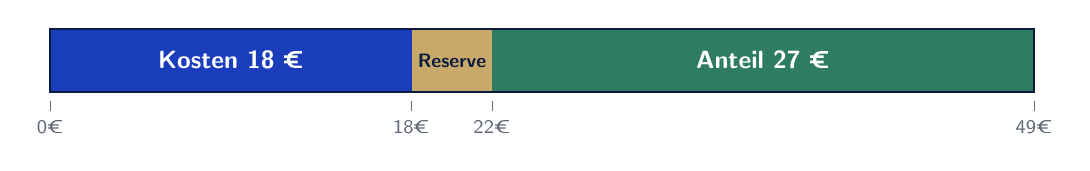
\begin{tikzpicture}[x=2.55mm,y=8mm]
  \fill[NordBlue] (0,2) rectangle (18,3);
  \fill[NordGold] (18,2) rectangle (22,3);
  \fill[NordGreen] (22,2) rectangle (49,3);
  \node[white,font=\sffamily\bfseries\small] at (9,2.5) {Kosten 18 €};
  \node[NordNavy,font=\sffamily\bfseries\scriptsize] at (20,2.5) {Reserve};
  \node[white,font=\sffamily\bfseries\small] at (35.5,2.5) {Anteil 27 €};
  \draw[NordNavy,thick] (0,2) rectangle (49,3);
  \foreach \x/\lab in {0/0,18/18,22/22,49/49} {
    \draw[NordMuted] (\x,1.85) -- (\x,1.7);
    \node[below,font=\sffamily\scriptsize\color{NordMuted}] at (\x,1.7) {\lab €};
  }
\end{tikzpicture}
\end{center}

\begin{tabularx}{\textwidth}{L{52mm}Y R{31mm}}
  \toprule
  \rowcolor{NordNavy}
  \color{white}\sffamily\bfseries Baustein &
  \color{white}\sffamily\bfseries Funktion &
  \color{white}\sffamily\bfseries monatlich \\
  Externe Kosten & Pro-Hosting und normale KI-Nutzung, gerundet & \eur{18,00} \\
  Variable Reserve & Wechselkurs, kleine Mehrnutzung, Blob- und API-Schwankungen & \eur{4,00} \\
  Persönlicher Anteil & Betriebsverantwortung, Administration, Risiko und Gewinn vor Steuern & \eur{27,00} \\
  \midrule
  \sffamily\bfseries Kundenpreis netto & \sffamily\bfseries monatliche Betriebspauschale & \sffamily\bfseries\eur{49,00} \\
  \bottomrule
\end{tabularx}

\textbf{Jahreswerte:}

\begin{itemize}
  \item Umsatz netto: \eur{588,00}
  \item Externes Kostenbudget: \eur{216,00}
  \item Variable Reserve: \eur{48,00}
  \item Persönlicher Deckungsbeitrag: \eur{324,00}
  \item Deckungsbeitragsquote: rund 55,1 Prozent
\end{itemize}

Der Deckungsbeitrag ist kein Nettogewinn nach Einkommensteuer, Gewerbesteuer, Zahlungsgebühren oder eigener Arbeitszeit. Er ist der Betrag, der nach der internen Kosten- und Risikoreserve wirtschaftlich übrig bleibt.

\subsection{Warum nicht günstiger als 49 Euro?}

Ein Preis von \eur{25} würde im empfohlenen Pro-Betrieb nur rund \eur{7} vor Arbeitszeit und Steuern übrig lassen. Schon ein kleiner Neon-Upgradebedarf würde die Marge aufzehren. Ein Preis von \eur{39} wäre möglich, ließe im Basisszenario aber nur rund \eur{17} nach Reserve. \eur{49} bleibt für einen Verein moderat, ist rund, einfach zu kommunizieren und übersteht einen einzelnen größeren Tarifsprung.

\subsection{Warum nicht sofort höher?}

Die realen Speicher- und Datenbankmengen sind sehr klein. Resend und Neon passen noch deutlich in die freien Kontingente. Ein höherer Preis wäre erst bei tatsächlich vereinbarter Wartungszeit, regelmäßigen Backups, garantierten Reaktionszeiten oder weiteren Funktionen sachlich besser zu begründen.

\begin{decisionbox}
  \textbf{Empfehlung:} \eur{49,00} netto monatlich ab dem Wechsel auf Vercel Pro. Abrechnung, Starttermin und Laufzeit werden separat vereinbart. Bei 19 Prozent Umsatzsteuer beträgt der Zahlbetrag \eur{58,31}; ohne Umsatzsteuer bleibt es bei \eur{49,00}. Der Preis enthält keine unbegrenzte Weiterentwicklung.
\end{decisionbox}

\section{Schutzklauseln für eine wirtschaftliche Pauschale}

Die folgenden Regeln verhindern, dass aus einer günstigen Pauschale eine unbegrenzte Kostenübernahme wird:

\begin{enumerate}
  \item \textbf{Normalnutzung:} Der Preis gilt für den üblichen Betrieb der Vereinswebsite, das Kontaktformular, CMS-Uploads und den Nord-Assistenten.
  \item \textbf{Anbietermehrkosten:} Zusätzliche verbrauchsabhängige Anbieterrechnungen über \eur{5} in einem Monat werden zunächst aus der Reserve getragen.
  \item \textbf{Preisprüfung:} Eine Anpassung wird ausgelöst, wenn externe Kosten in zwei aufeinanderfolgenden Monaten über \eur{25} liegen oder einmalig \eur{35} überschreiten.
  \item \textbf{Vorabinformation:} Ein planmäßiger Wechsel auf Neon Launch, Resend Pro oder einen anderen kostenpflichtigen Dienst erfolgt nur nach Information des Kunden.
  \item \textbf{Missbrauch:} Automatisierter, missbräuchlicher oder außergewöhnlicher KI-Traffic ist nicht unbegrenzt inklusive. Technische Schutzmaßnahmen dürfen ohne Funktionsverlust aktiviert werden.
  \item \textbf{Weiterentwicklung:} Neue Seiten, Funktionen, Datenmigrationen und größere Inhaltspflege werden separat angeboten.
  \item \textbf{Steuerklausel:} Gesetzliche Umsatzsteuer wird nur ausgewiesen, wenn sie tatsächlich anfällt.
\end{enumerate}

\section{Operative Maßnahmen vor Start der Abrechnung}

\begin{longtable}{@{}L{8mm}L{45mm}L{80mm}L{24mm}@{}}
  \toprule
  \rowcolor{NordNavy}
  \color{white}\sffamily\bfseries Nr. &
  \color{white}\sffamily\bfseries Maßnahme &
  \color{white}\sffamily\bfseries Begründung &
  \color{white}\sffamily\bfseries Priorität \\
  \endfirsthead
  \toprule
  \rowcolor{NordNavy}
  \color{white}\sffamily\bfseries Nr. &
  \color{white}\sffamily\bfseries Maßnahme &
  \color{white}\sffamily\bfseries Begründung &
  \color{white}\sffamily\bfseries Priorität \\
  \endhead
  1 & Vercel auf Pro umstellen & Beseitigt die Hobby-Nutzung als unsichere Grundlage eines bezahlten Kundenbetriebs. & sofort \\
  2 & OpenAI-Budgetlimit setzen & Begrenzung eines missbräuchlichen Kostenanstiegs. & sofort \\
  3 & Chat serverseitig limitieren & Der öffentliche Endpunkt besitzt heute kein Rate Limit. & sofort \\
  4 & Neon- und Resend-Tarif prüfen & Die Kalkulation nimmt Free an, aktuelle Kontorechnungen wurden nicht eingesehen. & vor Angebot \\
  5 & Vereins-Resend einrichten & Trennt Kundenbetrieb und Entwicklerdomain sauber. & kurzfristig \\
  6 & Kontenverantwortung festhalten & Regelt Zugang, Kündigung, Zahlungsweg und Übergabe. & vor Vertrag \\
  7 & Backup-Konzept umsetzen & Aktuell gibt es keine eigene, geprüfte Datenbanksicherung. & kurzfristig \\
  8 & Monatlichen Kostencheck führen & Vercel, Neon, Resend und OpenAI jeweils mit Istwert dokumentieren. & monatlich \\
  9 & Preisgrenze überwachen & Ab \eur{25} externen Kosten greift die vereinbarte Preisprüfung. & monatlich \\
  \bottomrule
\end{longtable}

\section{Monatliches Controlling}

Eine einfache monatliche Kontrolle von zehn Minuten reicht für den heutigen Umfang:

\begin{tabularx}{\textwidth}{L{37mm}Y L{38mm}}
  \toprule
  \rowcolor{NordNavy}
  \color{white}\sffamily\bfseries Prüffeld &
  \color{white}\sffamily\bfseries Kennzahl &
  \color{white}\sffamily\bfseries Warnschwelle \\
  Vercel & tatsächliche Rechnung, Nutzungsguthaben, Transfer, Function-Nutzung & Zusatzrechnung größer \eur{3} \\
  Blob & GB, Datentransfer, Zahl der Dateien & Wachstum größer 50 Prozent zum Vormonat \\
  Neon & CU-Stunden, Speicher, Transfer & 80 Prozent eines Free-Limits \\
  Resend & E-Mails pro Monat und Spitzentag & 2.400 monatlich oder 80 täglich \\
  OpenAI & Monatsbetrag und Zahl der Antworten & \eur{3} Warnung, \eur{5} harte Prüfung \\
  Verfügbarkeit & relevante Fehler und Ausfälle & wiederholter Fehler eines externen Dienstes \\
  \bottomrule
\end{tabularx}

Es genügt, die Werte in einer kleinen Tabelle mit Monat, Anbieter, Betrag, Nutzung und Bemerkung zu führen. Sobald belastbare Istwerte aus drei Monaten vorliegen, sollte die Reserve neu kalibriert werden.

\section{Leitlinie für die Kundenkommunikation}

Die Kundenfassung soll den Preis nachvollziehbar machen, ohne interne Kostenblöcke oder Margen offenzulegen. Entscheidend sind vier Aussagen:

\begin{tabularx}{\textwidth}{L{36mm}Y}
  \toprule
  \rowcolor{NordNavy}
  \color{white}\sffamily\bfseries Botschaft &
  \color{white}\sffamily\bfseries Begründung \\
  Professionelle Tarifbasis & Ein bezahlter Kundenbetrieb sollte nicht dauerhaft auf einem persönlichen Hobby-Tarif beruhen. \\
  Ein fester Gesamtpreis & Der Verein erhält Planbarkeit über Hosting, Datenbank, Medienspeicher, Mailversand, KI-Nutzung und Anbieterverwaltung. \\
  Angemessene Dimensionierung & Die heutigen Datenmengen sind klein. Deshalb ist kein teurer Enterprise-Tarif nötig. \\
  Klare Leistungsgrenze & Neue Funktionen, größere Inhaltspflege und spätere kostenpflichtige Tarifwechsel werden vorab abgestimmt. \\
  \bottomrule
\end{tabularx}

\begin{decisionbox}
  Die separate Kundenunterlage \textbf{„Vorschlag für den technischen Betrieb“} setzt diese Logik auf vier Seiten um. Sie nennt \eur{49,00} netto monatlich und \eur{588,00} netto jährlich, enthält jedoch weder persönlichen Deckungsbeitrag noch interne Reserven.
\end{decisionbox}

\section{Fazit}

Die Anwendung ist im Verhältnis zu ihrem Funktionsumfang kosteneffizient. Datenbank, Medien und E-Mail liegen weit unter den freien Kontingenten. Selbst die KI kostet im Normalfall nur wenige Cent bis deutlich unter einen Euro. Der relevante Fixkostenblock entsteht durch den empfohlenen Wechsel von Vercel Hobby auf Pro.

Mit \eur{49,00} netto monatlich entsteht ein einfaches und robustes Modell:

\begin{itemize}
  \item externe Normalkosten und Wechselkursschwankungen sind gedeckt,
  \item ein einzelnes größeres Upgrade kann zeitweise aufgefangen werden,
  \item ein persönlicher Deckungsbeitrag von \eur{27,00} monatlich bleibt planbar,
  \item der Kunde erhält einen klaren Festpreis ohne Einblick in interne Margen,
  \item ungewöhnliches Wachstum wird durch transparente Schwellen abgefangen.
\end{itemize}

\begin{decisionbox}
  {\sffamily\Large\bfseries\color{NordNavy}Finale Empfehlung}

  \textbf{\eur{49,00} netto pro Monat} für den technischen Betrieb. Start erst nach Prüfung der tatsächlichen Neon- und Resend-Tarife, Wechsel auf Vercel Pro und Einrichtung eines OpenAI-Kostenlimits. Größere Weiterentwicklungen bleiben separat vergütet.
\end{decisionbox}

\newpage
\section*{Quellen und Prüfpfade}
\addcontentsline{toc}{section}{Quellen und Prüfpfade}

Alle Onlinequellen wurden am 22.08.2026 abgerufen.

\begin{enumerate}
  \item Vercel Pricing, Hobby \eur{0}, Pro \usd{20}, Hobby für persönliche und nicht kommerzielle Nutzung: \url{https://vercel.com/pricing}
  \item Vercel Hobby Plan und enthaltene Nutzung: \url{https://vercel.com/docs/plans/hobby}
  \item Vercel Pro Plan, Plattformgebühr und \usd{20} Nutzungsguthaben: \url{https://vercel.com/docs/plans/pro-plan}
  \item Vercel regionale Preise für Blob, Transfer und Operationen: \url{https://vercel.com/docs/pricing/regional-pricing}
  \item Vercel Fluid Compute Pricing: \url{https://vercel.com/docs/functions/usage-and-pricing}
  \item Neon Pricing, Free und Launch: \url{https://neon.com/pricing}
  \item Resend Pricing: \url{https://resend.com/pricing}
  \item Resend Quoten und Limits: \url{https://resend.com/docs/knowledge-base/account-quotas-and-limits}
  \item OpenAI, Modell und Tokenpreise für \texttt{gpt-4o-mini}: \url{https://developers.openai.com/api/docs/models/gpt-4o-mini}
  \item Payload Self-Hosting und MIT-Lizenz: \url{https://payloadcms.com/get-started}
  \item OpenFreeMap, kostenlose öffentliche Instanz und fehlende SLA: \url{https://openfreemap.org/}
  \item BFV Nutzungsbedingungen, kostenlose Online-Daten und Vereins-Widgets: \url{https://www.bfv.de/allgemein/nutzungsbedingungen}
  \item ECB Referenzkurs vom 21.08.2026: \url{https://www.ecb.europa.eu/stats/policy_and_exchange_rates/euro_reference_exchange_rates/html/index.en.html}
\end{enumerate}

\textbf{Lokale Prüfpfade im Repository:}

\begin{itemize}
  \item \texttt{app/(frontend)/api/chat/route.ts}: Modell, Nachrichtenlimits und OpenAI-Aufruf
  \item \texttt{lib/ai-system-prompt.ts}: Größe und Inhalt des Systemprompts
  \item \texttt{payload.config.ts}: Neon- und Blob-Anbindung
  \item \texttt{app/(frontend)/api/contact/route.ts}: Resend-Pfad und Speicherung
  \item \texttt{lib/bfv.ts}, \texttt{lib/fupa.ts}, \texttt{lib/clubshop.ts}: externe Datenquellen
  \item \texttt{components/MapEmbed.tsx}: MapLibre und OpenFreeMap
  \item \texttt{OFFENE-PUNKTE.md}: Kontenlage und fehlende geprüfte Datenbanksicherung
\end{itemize}

\textbf{Produktivmessungen am 22.08.2026:}

\begin{itemize}
  \item Vercel API und CLI: Projekt \texttt{nord-lerchenau}, Tarif Hobby, Region \texttt{iad1}
  \item Vercel Blob CLI: 486 Dateien und 28.408.192 Byte
  \item Read-only PostgreSQL-Abfrage: Datenbankgröße 12 MB und 47 Tabellen
\end{itemize}

\vfill
\begin{center}
  \sffamily\footnotesize\color{NordMuted}
  Diese Ausarbeitung ist eine kaufmännische Planung und keine Steuer-, Rechts- oder Vertragsberatung.\\
  Anbieterpreise und Wechselkurse können sich ändern.
\end{center}

\end{document}
